
%%%%%%%%%%%%%%%%%%%%%%%%%%%%%%%%%%%%%%%%%%%%%%%%%%%%%%
%Figure
%%%%%%%%%%%%%%%%%%%%%%%%%%%%%%%%%%%%%%%%%%%%%%%%%%%%%%



\begin{figure}[H]
	\caption{Example of simple signature page with a single bank \newline
		The red circles indicate information extracted by the text search algorithm. This information includes the name and role of the bank, as well as the name and title of the signatory. The names of the banker, corporation, and corporate executive are anonymized for the sake of privacy. The prior literature offers additional, detailed descriptions of the data, as well as extensive quality checks \citep[e.g.][]{Herpfer.2018, Bushman2019}.}
	\label{fig:signature}
	\centering
	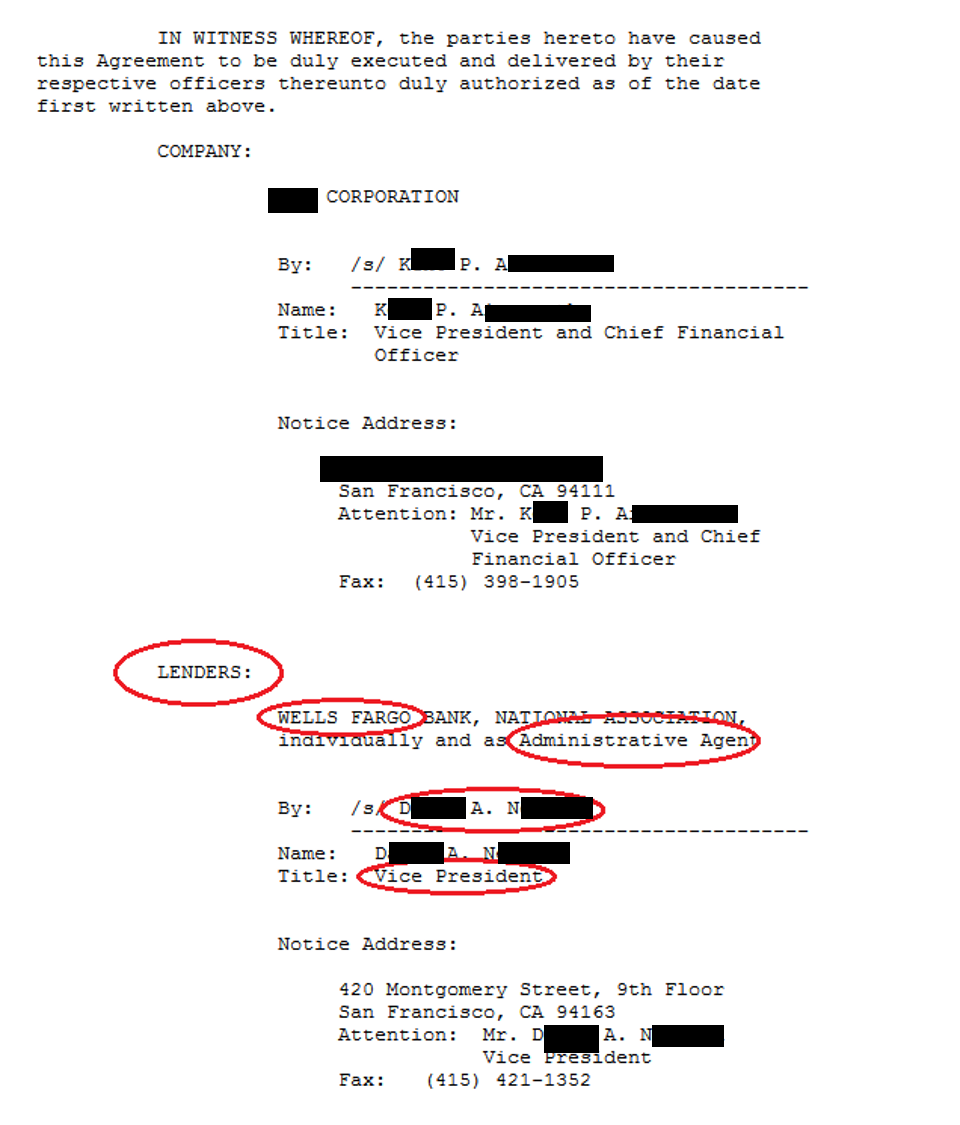
\includegraphics[angle=0,  scale=0.8]{figures/signature_well_formated.png}
\end{figure}

\clearpage \newpage

\begin{figure}[H]
	\caption{\textbf{Active bankers over time} \newline
		The figure shows the total number of active bankers in the sample (red line) and the cumulative number of bankers that switched and are still active (green line). Bankers are considered active for all years between the first and last deal they sign.}
	\label{fig:no_bankers}
	\centering
	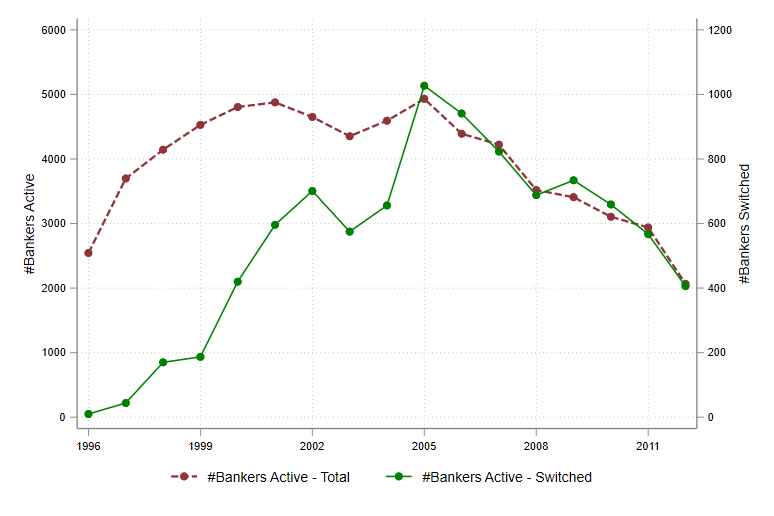
\includegraphics[angle=0,  scale=0.6]{figures/active_bankers_over_time.png}
\end{figure}
\clearpage \newpage

\begin{figure}[H]
	\caption{\textbf{Relationships acquired and initiations over time} \newline
		The figure shows the average yearly percentage of clients with whom a bank initiates a business relationship and for whom a personal relationship has been acquired. The x-axis show the number of years that elapsed since acquiring the relationship.
\textcolor{red}{CH: I am so sorry to keep pestering you about this graph but it still is not looking the way I have it in my head (and I am really stubborn :) ). This line should never go down. Right now, I understand the line some times goes down because some bankers are leaving the sample. I do not think that should happen if the data is constructed the way I think it is? Say we have some observations that took the value "initiation = 1, rel\_acq = 1". then the banker leaves the sample because she was inactive for 5 years (right? this is why the line only ever drops after 5 years?) But then initiation =1 and rel\_acq = 0? }	
}
	\label{fig:no_bankers}
	\centering
	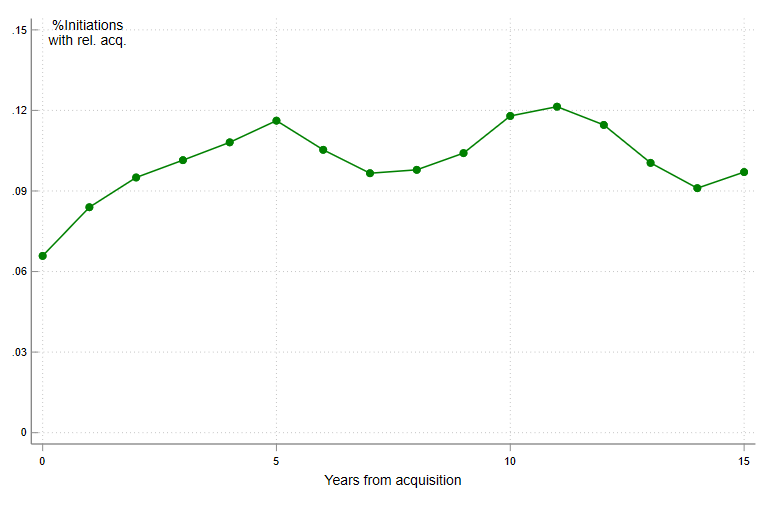
\includegraphics[angle=0,  scale=0.6]{figures/intiation_over_time.png}
\end{figure}



%
%%%%%%%%%%%%%%%%%%%%%%%%%%%%%%%%%%%%%%%%%%%%%%%%%%%%%%%
%Figure
%%%%%%%%%%%%%%%%%%%%%%%%%%%%%%%%%%%%%%%%%%%%%%%%%%%%%%%
%\begin{landscape}
%
%\begin{figure}[H]
%	\caption{Treatment dynamics (all deals) \newline
%		The figure presents the dynamics of treatment over time. Outcome variable is the log of dealsize across all three categories (loans, bonds, SEOs). Vertical bars represent 90\% confidence intervals for standard errors clustered at firm and lender. The year of treatment is the first year in which a banker appears on a loan for a new bank.} 
%	\label{fig:dynamics_full}
%	\centering
%	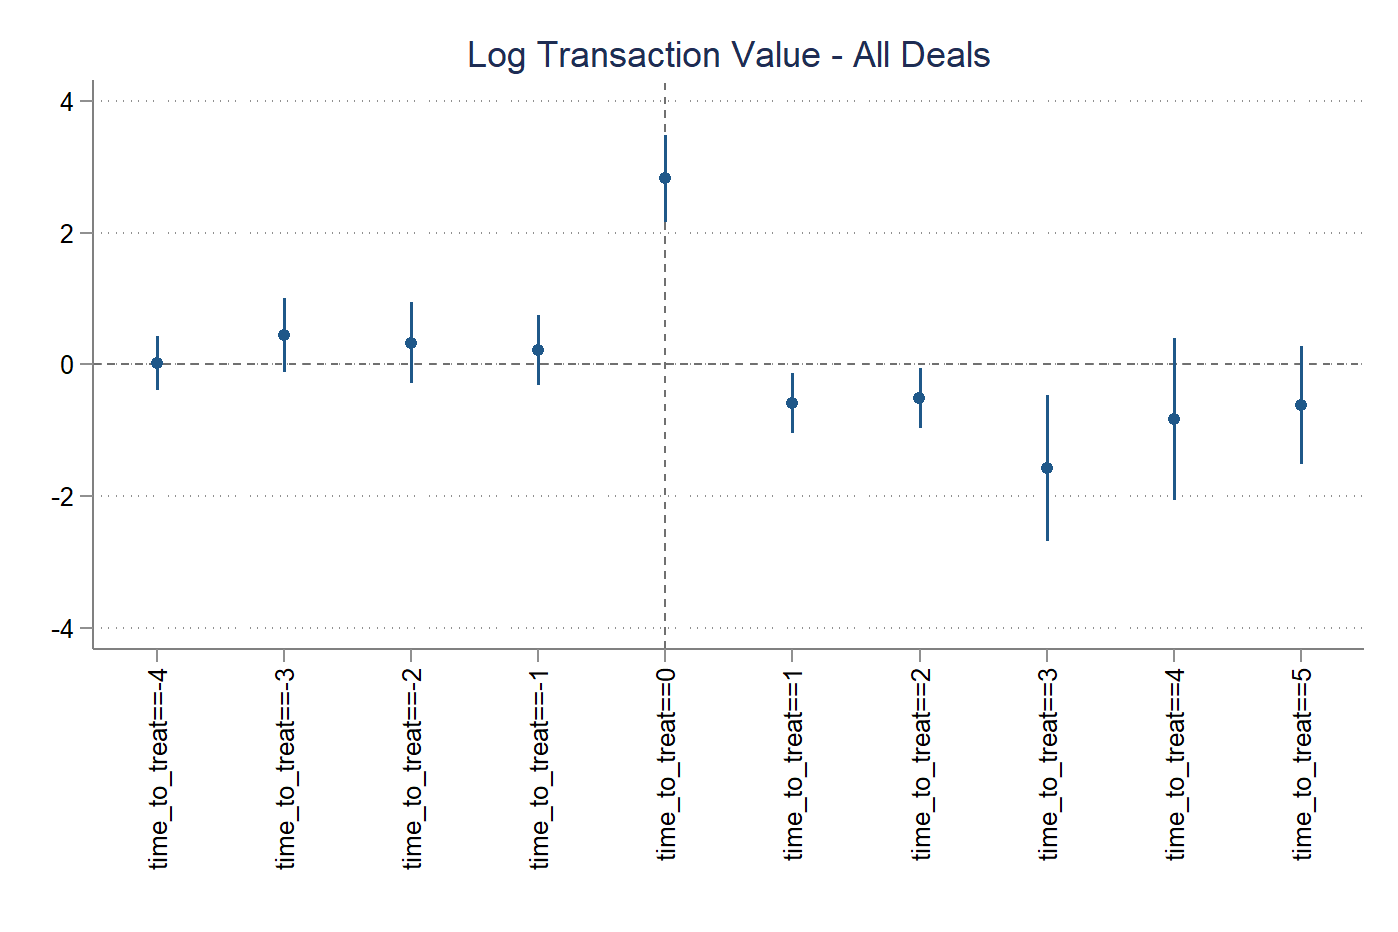
\includegraphics[angle=0,  scale=0.35]{figures/dynamics_logdealsize.png}
%\end{figure}
%\end{landscape}
%
%\clearpage \newpage
%%


%%%%%%%%%%%%%%%%%%%%%%%%%%%%%%%%%%%%%%%%%%%%%%%%%%%%%%%
%Figure
%%%%%%%%%%%%%%%%%%%%%%%%%%%%%%%%%%%%%%%%%%%%%%%%%%%%%%%
%
%\begin{figure}[H]
%	\caption{Treatment dynamics  (bonds only) \newline
%		The figure presents the dynamics of treatment over time. Outcome variable is the log of dealsize of new bonds issued. Vertical bars represent 90\% confidence intervals for standard errors clustered at firm and lender. The year of treatment is the first year in which a banker appears on a loan for a new bank.} 
%	\label{fig:dynamics_bonds}
%	\centering
%	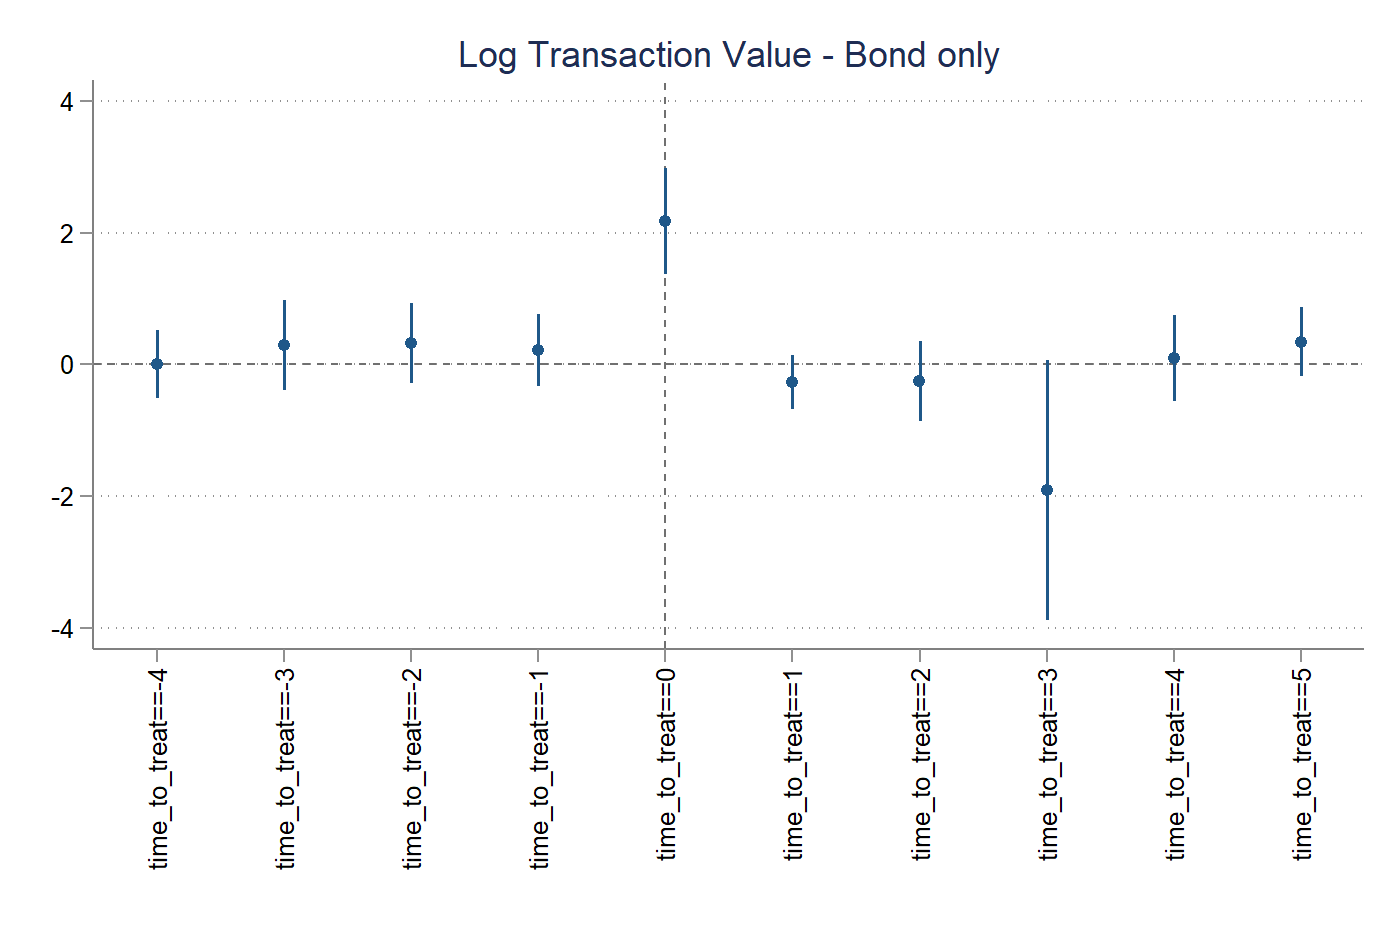
\includegraphics[angle=0,  scale=0.35]{figures/dynamics_logdealsize_bondonly.png}
%\end{figure}
%\end{landscape}
%
%\clearpage \newpage
%
%%%%%%%%%%%%%%%%%%%%%%%%%%%%%%%%%%%%%%%%%%%%%%%%%%%%%%%
%Figure
%%%%%%%%%%%%%%%%%%%%%%%%%%%%%%%%%%%%%%%%%%%%%%%%%%%%%%%
%
%
%\begin{figure}[H]
%	\caption{Treatment dynamics (SEO only) \newline
%		The figure presents the dynamics of treatment over time. Outcome variable is the log of dealsize of seasoned equity offerings. Vertical bars represent 90\% confidence intervals for standard errors clustered at firm and lender. The year of treatment is the first year in which a banker appears on a loan for a new bank.} 
%	\label{fig:dynamics_seo}
%	\centering
%	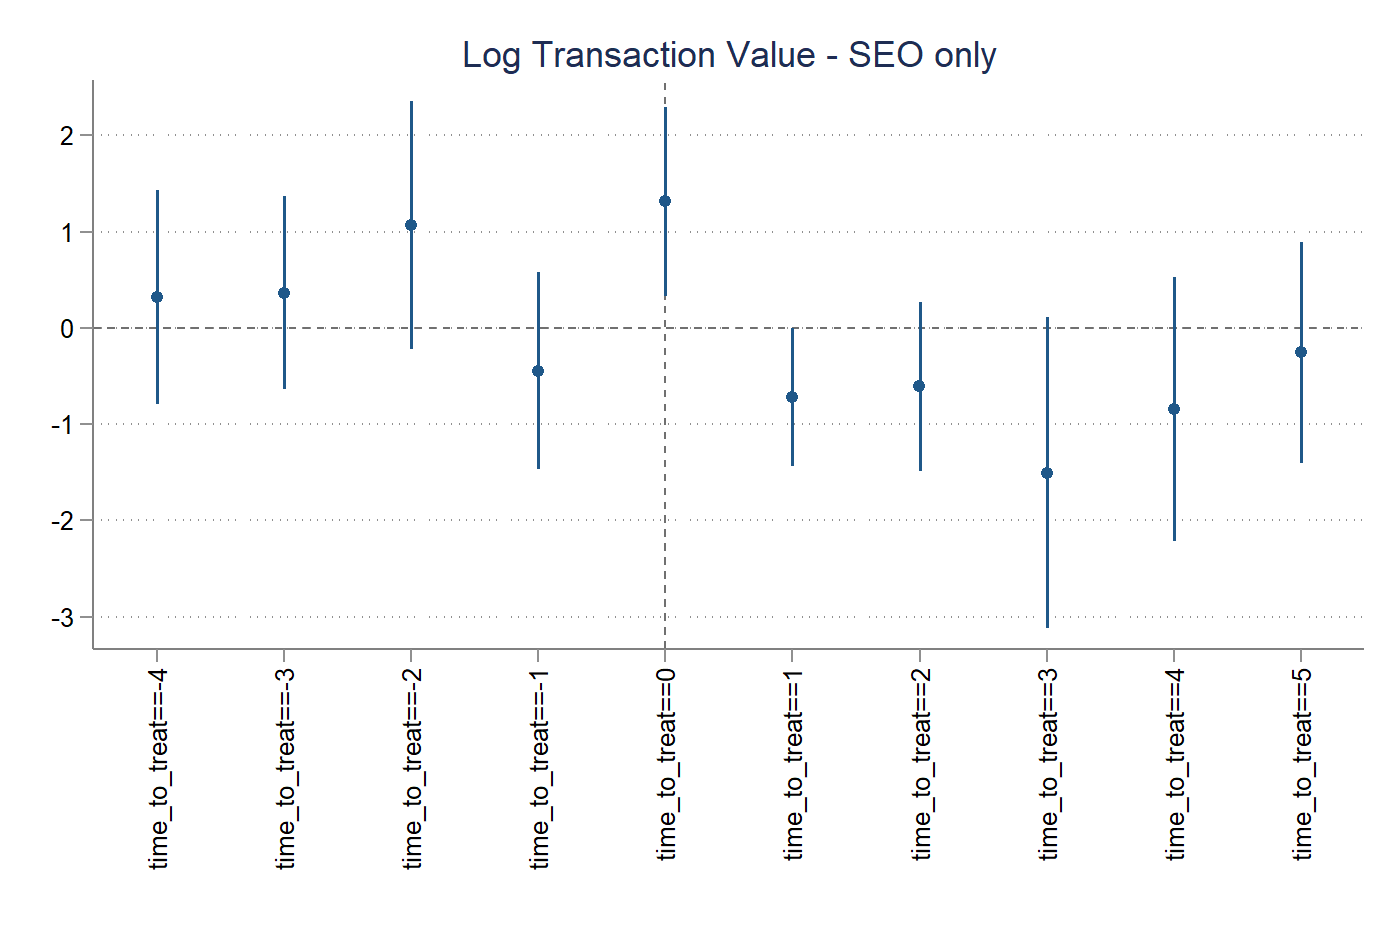
\includegraphics[angle=0,  scale=0.35]{figures/dynamics_logdealsize_seoonly.png}
%\end{figure}
%\end{landscape}
%
%\clearpage \newpage
%
%\begin{figure}[H]
%\captionsetup[subfigure]{justification=centering}
%	\centering
%	\caption{\textbf{Treatment dynamics - First deal and repeat business} \newline The figure presents the dynamics of treatment over time. Outcome variable in Panel A is the log of dealsize of the first deal (either syndicated loan, bond underwriting, or seasoned equity offering) in which a banker appears on a loan for a new bank. Panel B shows the total transaction value of repeated business done with a client (except for the first deal). Vertical bars represent 90\% confidence intervals for standard errors clustered at firm and lender. The year of treatment is the first year in which a banker appears on a loan for a new bank.} 
%	\label{fig:dynamics_first_repeated}
%	\begin{subfigure}[H]{\textwidth}
%		\centering
%		\caption*{\textbf{Panel A:} Log Transaction Value - First deal of old clients at new bank}
%		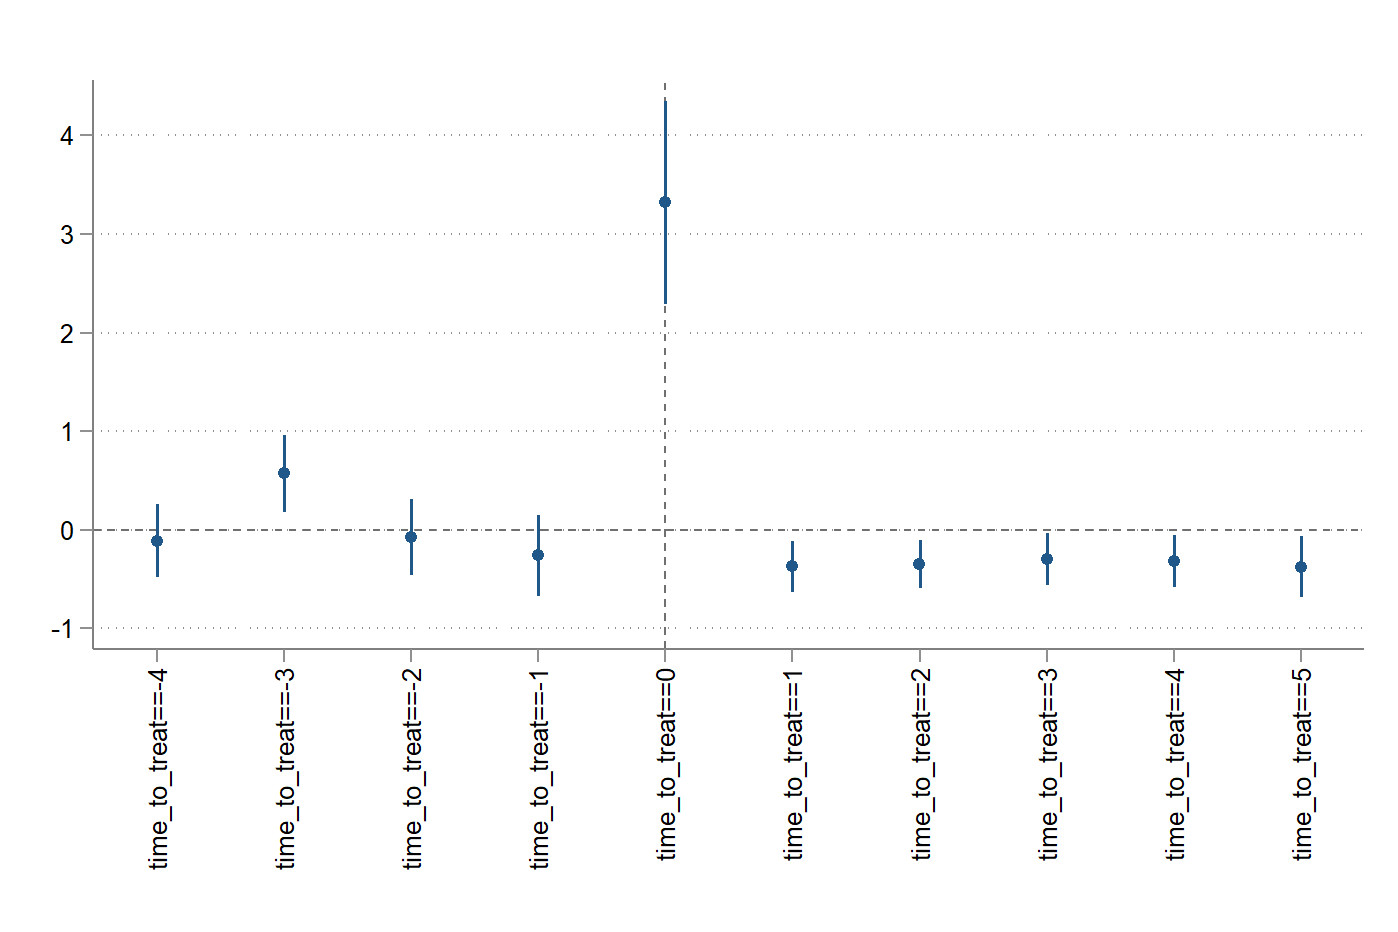
\includegraphics[angle=0,  scale=0.3]{figures/dynamics_logdealsize_firsttime.png}
%		\caption*{[Continued on the next page]}
%	\end{subfigure} \end{figure}
%
%\begin{figure}[H]
%\captionsetup[subfigure]{justification=centering}
%	{\small \centering [Continued from previous page] \\ ~ \newline}
%	\begin{subfigure}[H]{\textwidth}
%		\centering
%		\caption*{\textbf{Panel B:} Log Transaction Value - Repeat business with old clients at new bank}
%		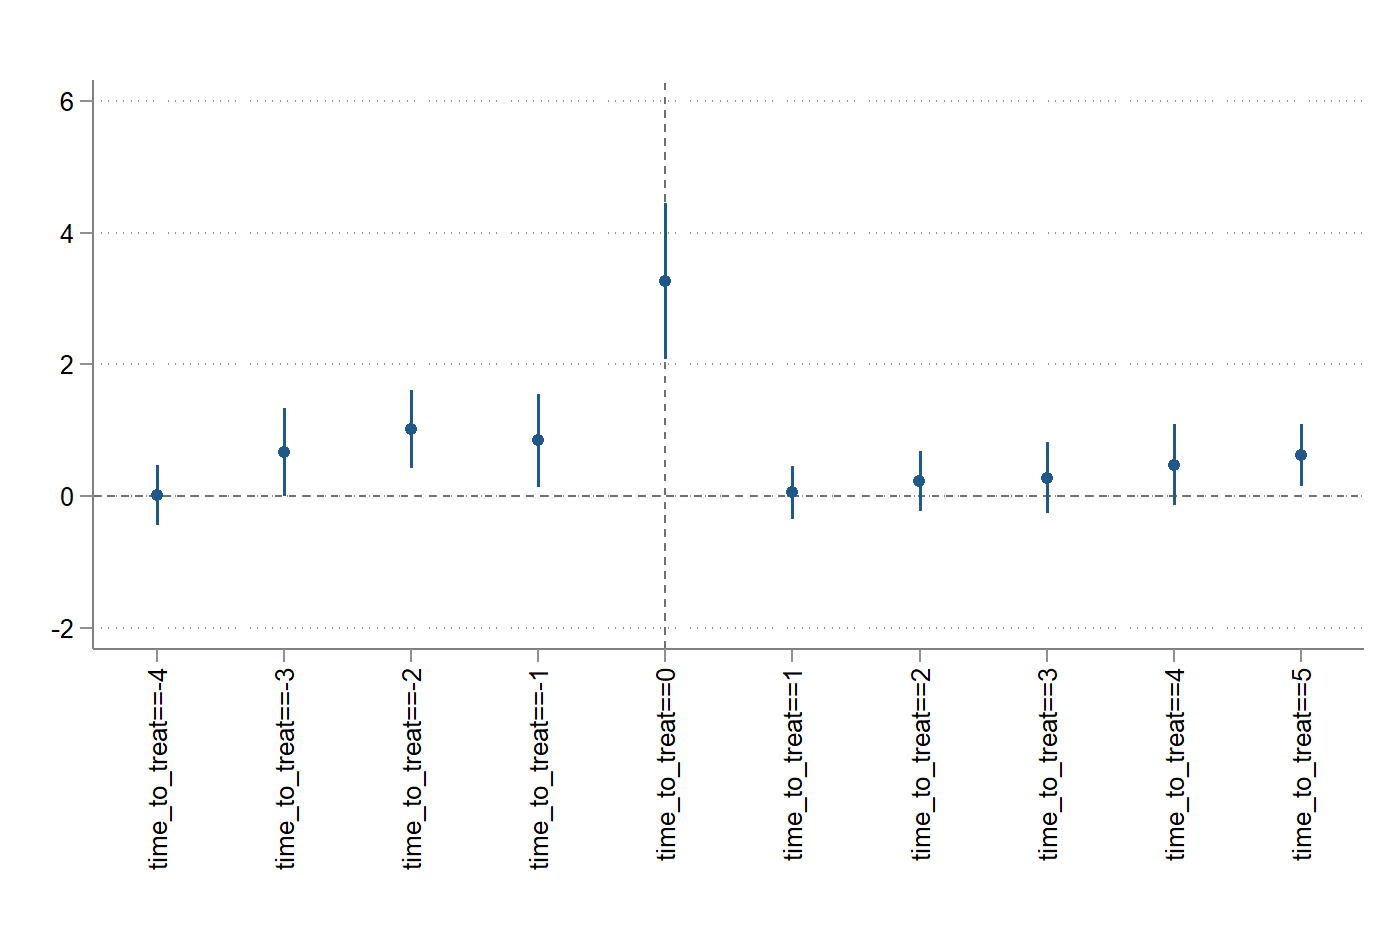
\includegraphics[angle=0,  scale=0.3]{figures/dynamics_logdealsize_repeat.png}
%	\end{subfigure}
%\end{figure}
%
%%%%%%%%%%%%%%%%%%%%%%%%%%%%%%%%%%%%%%%%%%%%%%%%%%%%%%%
%Figure
%%%%%%%%%%%%%%%%%%%%%%%%%%%%%%%%%%%%%%%%%%%%%%%%%%%%%%%